% Geometry of the two periodic leads and the line defect in Section 2.1.
\begin{figure}[htbp]
\centering
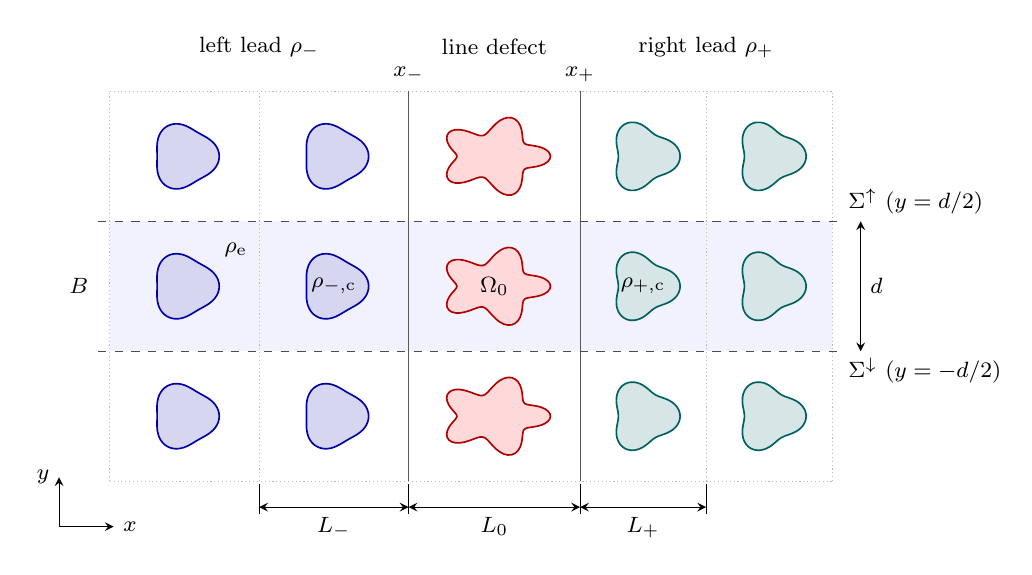
\begin{tikzpicture}[x=1.65cm,y=1.65cm,font=\footnotesize,>=stealth,
  cell wall/.style={gray!55,densely dotted,thin},
  seam/.style={black!70,dashed,thin},
  measure/.style={<->,thin},
  pics/lead rod/.style args={#1/#2}{code={
    \filldraw[draw=#1,fill=#1!16,line width=.6pt]
      plot[domain=0:360,samples=73,variable=\t]
      ({.24*(1+#2*cos(3*\t))*cos(\t)/sqrt(1+#2*#2/2)},
       {.24*(1+#2*cos(3*\t))*sin(\t)/sqrt(1+#2*#2/2)}) -- cycle;}},
  pics/defect rod/.style={code={
    \filldraw[draw=red!70!black,fill=red!15,line width=.6pt]
      plot[domain=0:360,samples=91,variable=\t]
      ({.24*(1.5+.3*cos(5*\t))*cos(\t)},
       {.24*(1+.3*cos(5*\t))*sin(\t)}) -- cycle;}}]
  % Two full lead cells on each side; three transverse periods.
  \fill[blue!5] (-2.96,-.5) rectangle (2.60,.5);
  \foreach \x in {-2.96,-1.81,1.63,2.60}
    \draw[cell wall] (\x,-1.5) -- (\x,1.5);
  \foreach \y in {-1.5,1.5}
    \draw[cell wall] (-2.96,\y) -- (2.60,\y);
  \foreach \x in {-.66,.66}
    \draw[black!65,thin] (\x,-1.5) -- (\x,1.5);
  \foreach \y in {-.5,.5}
    \draw[seam] (-3.05,\y) -- (2.69,\y);
  \foreach \y in {-1,0,1} {
    \foreach \x in {-2.385,-1.235}
      \pic at (\x,\y) {lead rod={blue!65!black/.12}};
    \pic at (0,\y) {defect rod};
    \foreach \x in {1.145,2.115}
      \pic at (\x,\y) {lead rod={teal!75!black/.20}};
  }
  \node at (-1.81,1.84) {left lead $\rho_-$};
  \node at (0,1.84) {line defect};
  \node at (1.63,1.84) {right lead $\rho_+$};
  \node[above] at (-.66,1.5) {$x_-$};
  \node[above] at (.66,1.5) {$x_+$};
  \node at (0,0) {$\Omega_0$};
  \node at (-1.99,.28) {$\rho_{\mathrm e}$};
  \node at (-1.235,0) {$\rho_{-,\mathrm c}$};
  \node at (1.145,0) {$\rho_{+,\mathrm c}$};
  \node[left] at (-3.05,0) {$B$};
  \draw[measure] (2.82,-.5) -- node[right] {$d$} (2.82,.5);
  \node[above right,inner sep=1pt] at (2.70,.53)
    {$\Sigma^\uparrow\ (y=d/2)$};
  \node[below right,inner sep=1pt] at (2.70,-.53)
    {$\Sigma^\downarrow\ (y=-d/2)$};
  \foreach \a/\b/\period in {-1.81/-.66/L_-,-.66/.66/L_0,.66/1.63/L_+} {
    \draw[thin] (\a,-1.52) -- (\a,-1.75);
    \draw[measure] (\a,-1.70) -- node[below] {$\period$} (\b,-1.70);
  }
  \draw[thin] (1.63,-1.52) -- (1.63,-1.75);
  \draw[->] (-3.35,-1.85) -- ++(.42,0) node[right] {$x$};
  \draw[->] (-3.35,-1.85) -- ++(0,.38) node[left] {$y$};
\end{tikzpicture}
\caption{Two periodic leads separated by a line defect with center rod
$\Omega_0$. The rod boundaries form $\Upsilon$. The shaded row is one period
strip $B=\RR\times I_d$; translation from its lower edge to its upper edge
multiplies the field by $\ee^{\ii\beta d}$.}
\label{fig:model-geometry}
\end{figure}
